% !TEX root = ../calibreport.tex
%================================
The results of this section reports the estimation for the eight SUT given in the table \ref{tab:sensor-specifications}.
The analysis is on the data from IS26. Each query on the DB is on 2 consecutive days from the 1st of June to the 9th of October, saying about 130 days. For each file a spectral analysis is processed leading to an SUT response estimate. From the spectral components we perform, in each frequency band and for each time interval, the response of the system under test (SUT) using the known response of the reference sensor. These responses includes both the sensor and the digitizer. These responses are averaged over the full set of time intervals over the all days. The  MSC threshold is fixed to $0.98$. 

Let us remain the PTS specifications:
\begin{itemize}
\item
IMS pass-band requirement $[0.02 - 4]$ Hz;
 \item
$\pm 5\%$ on the response magnitude, i.e. $\pm 0.43$ in dB scale;
\item
the calibration is required at least once a year;
 \item
no requirement  on the phase but $\ldots$ $\pm 5\degree$ as for seismic requirements.
\end{itemize}


 \newpage
%================================
\section{Results of IS26 - sensor \#1}
%================================
In this section we only considered the sensor \#1, but identical results have be obtained on the seven other sensors.


%================================
\subsection{SUT response by averaging on $124$ days}
%================================
The average estimate of the SUT response, in terms of gain in dB and phase in degree, are reported figure \ref{fig:withoutproblemons1}. The red dashed lines report the theoretical SUT response range requirements, which is $\pm 0.43$ for the gain and $\pm 5\degree$ for the phase. They have be performed taking into account the SREF sensor response and using the model of NRS developped by the IMS.
\figscale{figures/withoutproblemons1.pdf}{The red dashed lines report the theoretical SUT response range requirement, which is $\pm 0.43$ for the gain and $\pm 5\degree$ for the phase.}{fig:withoutproblemons1}{0.8}

 \newpage\clearpage
%================================
\subsection{Using different thresholds on a pair of days}
%================================
\figscale{2daysonIS26SUT1year2015day152diffTH}{Sup ratio in dB given by the expression \eqref{eq:ratio-sup-bis-exact} for 2 successive days into the $P=6$ frequency bands for different values of the MSC threshold. The gray dots report the values associated to the MSC greater than the threshold. The color dots report the weighted averagings on the gray values. We see larger dispersion lower the MSC threshold. Also we see  differences between the associated averagings, meanind that a bias is present. Theoretically (under regular assumptions) the bias is larger for lower MSC threshold.}{}{0.8}


\newpage\clearpage
%================================
\subsection{More details on a pair of days}
%================================
\figscale{figures/2daysonIS26SUT1year2015day233.pdf}{Sup ratio in dB given by the expression \eqref{eq:ratio-sup-bis-exact} for 2 successive days into the $P=6$ frequency bands.}{}{0.8}

\figscale{figures/2daysonIS26SUT1year2015day233aboveTH.pdf}{Sup ratio in dB given by the expression \eqref{eq:ratio-sup-bis-exact} for 2 successive days into the $P=6$ frequency bands for MSC above the threshold. We observe a very few events in the frequency mid-ranges, in this case we have to use a very long period of time to reduce the dispersion.}{}{0.8}



\newpage\clearpage
%================================
\subsection{Problem with some records}
\label{ss:problems}
%================================
In this section we report a few issues we have observed in the recorded signals of the database {\tt tesbed\_archive} and that can be considered as "true" outliers.
In figure \ref{fig:withproblemons1} we have considered the same data than those of figure \ref{fig:withoutproblemons1}, adding two days more. These two days induce a burst in the performed SUT response. To identify the origin, we have plotted the signals of these two days figure \ref{fig:clickdetails1year2015day286aboveTH}. We clearly observed huge bursts in two samples locations. If we suppress these 2 bursts and re-introduce the two cleaned days to perform the SUT response, we obtain the curves reported \ref{fig:withproblemons1solved}, which are very similar to the curves figure \ref{fig:withoutproblemons1}. We may conclude than unusual values in the observed signals (outliers) lead to false measurement of the SUT response. Therefore it is very important to identify these outliers before any calibration.




\figscale{figures/withproblemons1.pdf}{Same data than those of figure \ref{fig:withoutproblemons1} but  adding two days more. We observe that a few values seem to be outliers. The data of these two days are reported figure \ref{fig:clickdetails1year2015day286aboveTH}. We see large bursts that are at the origin of the ouliers.}{fig:withproblemons1}{0.8}


\figscale{figures/clickdetails1year2015dayth1aboveTH.pdf}{Two days data added in the protocol to obtain the figure \ref{fig:withoutproblemons1}. We observe large bursts that can be considered as outliers, as they appear hugely greater than the observed values outside of the bursts.}{fig:clickdetails1year2015day286aboveTH}{1}

\figscale{figures/withproblemons1Solved.pdf}{Same data than those of figure \ref{fig:withproblemons1} but  suppressing the part of the added signals where  bursts are located. The figure is very similar to the figure \ref{fig:withoutproblemons1}.}{fig:withproblemons1solved}{0.8}

\newpage\clearpage
\subsubsection{Synchronization problem}
Another problem is the full desynchronization of the two sensor signals, as for example the 2015/08/09 on the sensor 1. A part of the trace is reported on figure \ref{fig:fillshift} but the shift is on the complete duration.

\figscale{figures/fillshift.pdf}{Time shift on the full duration.}{fig:fillshift}{0.8}

\newpage\clearpage
%================================
\subsection{Averaging on randomly selected pairs of days}
%================================


Let us remain that a malfunction of short duration can be regarded as an outlier and can be removed from the useful data. It follows that during an averaging of the estimated responses we can remove what happen very rarely. For this reason we suppress a short percent of the extreme values, which is less brutale than the median approach. This kind of averaging is often called trimmed mean.

Therefore to avoid the problems, cited section \ref{ss:problems}, which appear very rarely, it is advised to use a trimmed mean on several pairs of days. Figure \ref{fig:withtrimmeanonstation1}, randomly selected pairs of days are reported with a simple mean 
and a trimmed mean excluding $30\%$ of the lowest and highest values. We see that the outlier present in the red curves is suppressed automatically by the trimmed mean. This outlier is due to the data of the 13th of October in station 1 and at the origin of the clich we see on figure \ref{fig:withoutproblemons1}.   


\figscale{figures/withtrimmeanonstation1.pdf}{Sup ratio given by the expression \eqref{eq:ratio-sup-bis-exact}. The gray points report the ratios averaged on a pair of 2 consecutive days, the red points report the simple mean on 15 pairs of days, the blue  the trimmed mean excluding $30\%$ of the lowest and highest values}{fig:withtrimmeanonstation1}{0.8}

%================================
\newpage\clearpage
%================================
\subsection{Stability at different frequency values}
%================================

For different frequencies we draw randomly between the all pairs of days a certain number of them. We apply an averaging with trimming $20\%$ of the extreme values. The results are reported figure \ref{fig:averagingonagivenpairsofdays}.

At first we report figure \ref{fig:evolutionon1atfreq1Hz} the Sup ratio given by the expression \eqref{eq:ratio-sup-bis-exact} at 1 Hz for all pairs of successive days. Our database consists of $70$ pairs of days. The selected frequency is 1 Hz. It appears one point at the limit of the requirements of the PTS.

\figscale{figures/evolutionon1atfreq1Hz.pdf}{$140$ pairs of days have been studied between the $1$st of June to the $30$th October $2015$. Top: the value of theSup ratio at $1$ Hz in a range centered on the measures with a width of $\pm 5\%$. For thus duration of $48$ hours a few points are outside the range. Therefore the idea to average on a few pairs, e.g. figure \ref{fig:evolutionon1atdifffreq} the averaging is on 1 month. Bottom: the number of points over the threshold at the frequency of $1$ Hz. Some pairs of  days the number is only $1$. They correspond to the points in top figure outside of the requirement range. }{fig:evolutionon1atfreq1Hz}{0.8}

%================================
\newpage\clearpage

We repeat the same operations by taking $15$ pairs of days (i.e. $1$ month) at different frequencies and with a trimmed mean excluding the $30\%$ extreme values. We observe that the frequencies around the dip is a little bit more unstable. Complementary  results are given section \ref{ss:ciandstdsection}

\figscale{figures/evolutionon1atdifffreq.pdf}{Randomly draw in the sequence of pairs of days.}{fig:evolutionon1atdifffreq}{0.8}


%================================
\newpage\clearpage
%================================
%================================
\section{Comments}
%================================
\subsection{About the selected MSC threshold}
%================================
We said that we can not choose a too low value for the MSC threshold because the underdetermination. That appears clearly on figure \ref{fig:afewdaysonI26C6H6twoMSC}.
When the  MSC threshold is $0.7$, there is a large discrepancy between the estimated ratios, see \eqref{eq:estimated-Ratio} and we outline that there is no way to solve the underdetermination. But for an MSC threshold of $0.95$, the two curves are very close.

\figscale{afewdaysonI26C6H6twoMSC.pdf}{Couple H6C6, for two MSC thresholds.}{fig:afewdaysonI26C6H6twoMSC}{0.7}

On the other hand if the ratio between the two noise levels are perfectly known the indetermination is removed and we can use formula \eqref{eq:known-noise-ratio}. You might be tempted to say that the two noises on the two sensors are identical except theirs levels and consider that the ratio is given by the number of inlets in the noise reduction system. However the figure \ref{fig:afewdaysonI26C4H4knownnoiseratio} shows that the curve with a MSC threshold of $0.5$ and the formula \eqref{eq:known-noise-ratio} lead to values different from the curves obtained with a a MSC threshold of $0.95$.

\figscale{afewdaysonI26C4H4knownnoiseratio.pdf}{Couple H4C4, for two MSC thresholds with formula \eqref{eq:known-noise-ratio}.}{fig:afewdaysonI26C4H4knownnoiseratio}{0.7}

%================================
\newpage\clearpage
%================================
\subsection{Dip on the curves}
%================================
In all previous figures we observe an important dip around 0.1 Hz.  Also we have reported figure \ref{fig:afewdays1colocation} the ratio \eqref{eq:ratio-sup-bis-exact} for a few days on the location H2C2. The different colors are for different days. The distribution seems to be uniform and does not depend on the day. The ratio seems to be different of 1.\\*

If the MSC is about 0.99, meaning that the noises on the two sensors are negligible, and if the two sensors have the same response, the only reason to get a ratio less than 1, is that the acoustical SOI on the SUT is attenuated, may due to the noise system reduction. That would write: it exists $\alpha\in\mathbb{C}$ with $|\alpha|<1$ s.t.:
\begin{eqnarray}
\label{eq:model-of-obervation}
\left\{
\renewcommand\arraystretch{1.6}
\begin{array}{rcl}
x_{\ut}(t)&=&g_{\ut}  \star (\alpha s(t))
\\
x_{\rf}(t)&=&g_{\rf}  \star s(t)
\end{array}
\right.
\end{eqnarray}

\figscale{afewdays1colocation.pdf}{a few days on H2C2. Only the band $[0.08-0.12]$ Hz is selected. The coherence is above $0.99$. The different colors for the different days.}{fig:afewdays1colocation}{0.5}


Another way to see the response differences between the 2 sensors in the band  $[0.08-0.12]$ Hz (gain ratio different of 1), appears figure \ref{fig:filteredsignals}. A zoom of the signals is plotted. It consists of about 1 minute, around a position where the observed coherence is above $0.99$. We see that the signal on the SREF  is bigger than this on the SUT. There is no way and no reason to reject this time window since the difference can be due either to the loss of gain or a unknown transfer function. 
\begin{figure}%{20cm}
\begin{minipage}{10cm}
              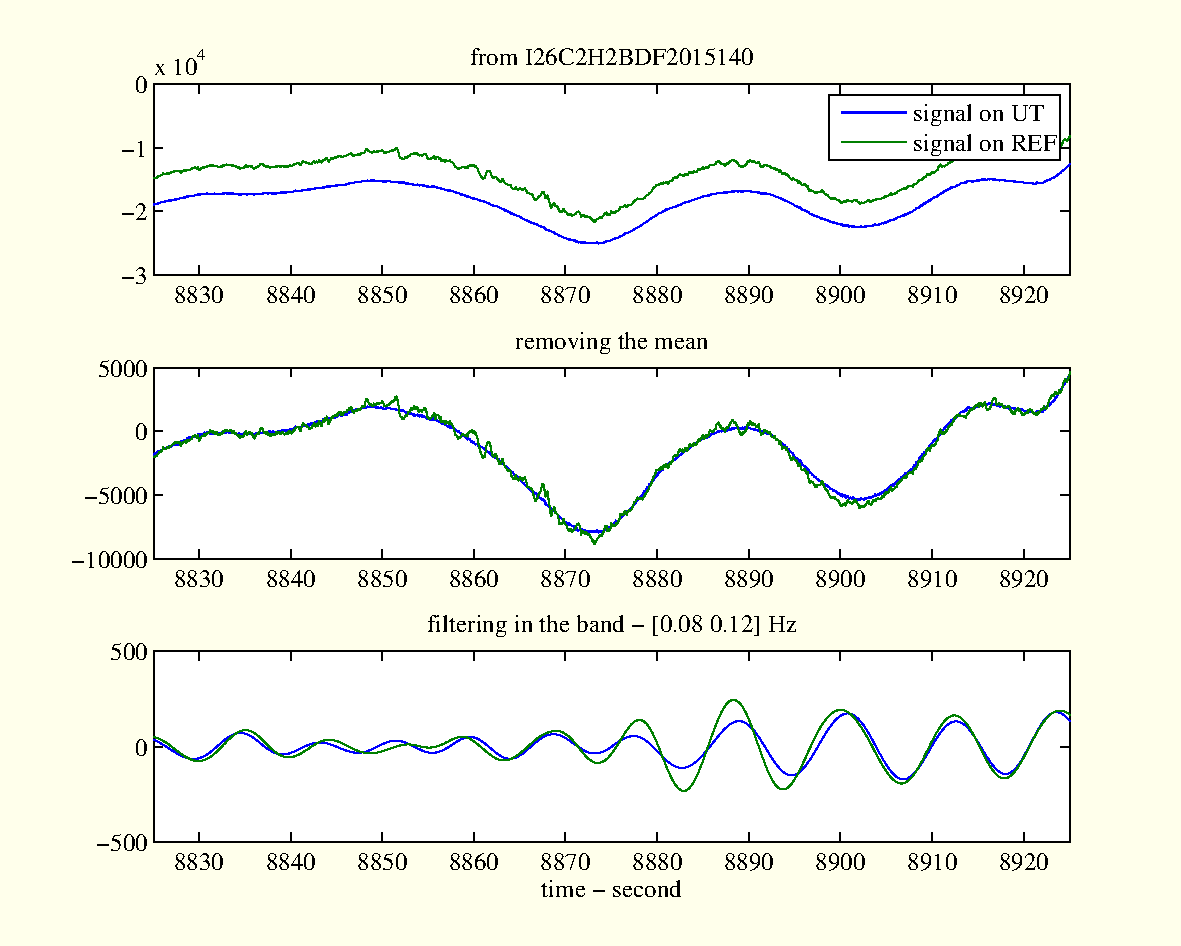
\includegraphics[scale=0.5]{signalsanomaly.pdf}
\end{minipage}
\begin{minipage}[c]{8cm}
              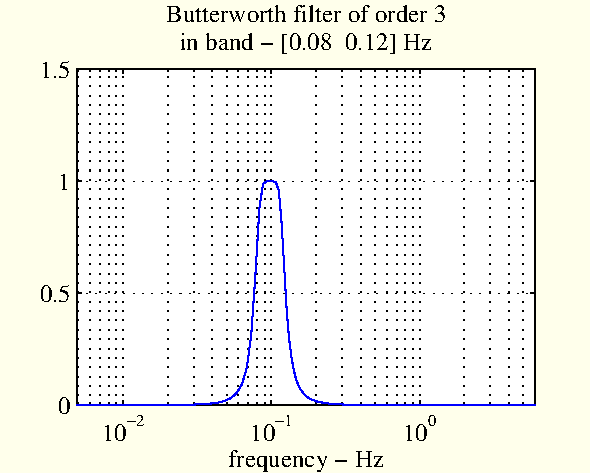
\includegraphics[scale=0.5]{filteranomaly.pdf}    

\end{minipage}
\centering
\caption{Filtered signals}
\label{fig:filteredsignals}
\end{figure}

